\Appendix{}

\label{appendix:B}

\section{Effect of Atom Replacement on the Polarizability of Polymers}

As discussed Chapter 2, the polarizability is highly dependent on the moieties that are incorporated into the polymer backbone or in the side chain. To examine this dependence, we replaced the atoms in the example polymer (thio-ene polymer) and observed the change in the polarizability. The list of atomic changes and the corresponding change in the polarizability is shown in the Table \ref{atom_dep}. We observe that the polarizability is highly dependent on the type of heteroatoms used in the monomer.


\begin{table}[]
	\centering
	\caption{Effect of replacing atoms on the polarizability of the thiol-ene monomer }
	\label{atom_dep}
	\begin{tabular}{ll}
		\hline
		Monomer type     & Polarizability α (bohr$^3$) \\ \hline
		Original monomer & 383.43                   \\
		S to O           & 317.20                   \\
		Si to C          & 358.75                   \\ 
		Si to Ge         & 393.32                   \\
		Si to Sn         & 418.33                  
	\end{tabular}
\end{table}

\section{Geometry Dependence of Polarizability}

Due to the complicated structure of the thiol-ene polymers, it is vital to understand the dependence of polarizability on the polymer geometry. To check this dependence, we performed a simple test. In this test, we changed the configuration of the aromatic moieties in the thiol-ene monomer as shown in the Fig.\ \ref{fig:geom_dep}(a). The strategy was to fix the angle between specific atoms in the two benzyl rings and then optimize the geometry. In the first case, we fixed the angle between carbon atoms labeled as 1, 2 and 3 (angle 123) and change the angle 234. Both the benzyl rings are aligned parallel in all the runs i.e the sum of angle 123 and angle 234 is 180$^0$. In the second case, one benzyl ring was fixed while the other benzyl ring orientation was changed. The polarizability changes in both these cases is shown in the Fig.\ \ref{fig:geom_dep}(b). The polarizability does not significantly change with the orientation of the aromatic moieties. Thus, the orientation of benzene rings does not play a significant role in the polarizability calculations of thiol-ene polymers. Further studies are needed to establish a detailed insight on the dependence of polarizability on the geometry. 

\begin{figure}[htbp] 
	\centering
	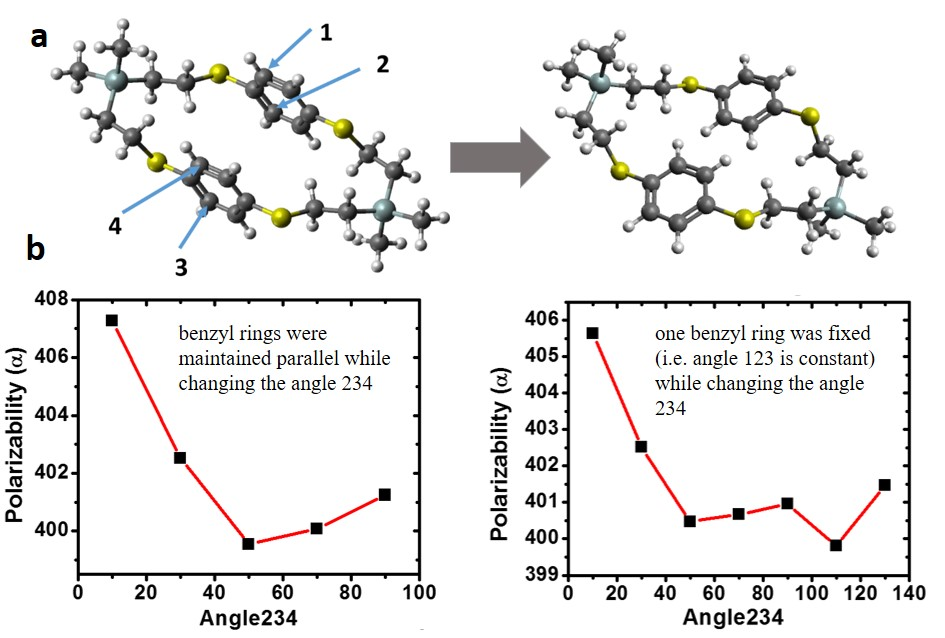
\includegraphics[width=0.95\textwidth]{Appendix-B/Figures/geom_dep.jpg}
	\caption{\textbf{(a)} Schematic of the change in the configuration of aromatic moieties in thiol-ene monomer, \textbf{(b)} the change in the polarizability with the orientation of aromatic moieties.} 
	\label{fig:geom_dep} 
\end{figure}


